\chapter{Planificación y presupuesto}

En el mundo de la gestión de proyectos, nos encontramos con varias etapas que guían el rumbo y éxito de cualquier iniciativa. Es un ciclo continuo con diversas fases interconectadas conocidas como el 'Ciclo de vida de un proyecto'. 

En esta sección haremos un recorrido comentando el ciclo de vida del proyecto, desglosando la planificación, y haciendo una estimación sobre el coste que supone el desarrollo del mismo.\vspace{0.3cm}

\section{Planificación}

La planificación de un proyecto tiene como objetivo su realización en las condiciones ideales y asegurando los mejores resultados. Este ciclo de vida es un marco conceptual que divide la evolución de un proyecto en etapas secuenciales, cada una con sus diferentes objetivos. Para el desarrollo de este proyecto se han seguido las siguientes etapas. 

\begin{itemize}
    \item \textbf{Estudio} de distintos tipos de chatbots y trabajos similares que nos servirán como ejemplo a la hora de definir la funcionalidad del proyecto. Realización de cursos y estudio de la documentación de las tecnologías que vamos a usar.
    \item \textbf{Documentación} de la memoria realizada concurrentemente en todas las etapas del proyecto. 
    \item \textbf{Análisis} del proyecto, identificando los requisitos, entidades y componentes, así como la forma de interactuar entre sí. 
    \item \textbf{Diseño} de la base de datos, generación de mockups para las interfaces de usuario y arquitectura. 
    \item \textbf{Implementación} del software teniendo en cuenta todo los aspectos estudiados en las etapas previas.
    \item \textbf{Evaluación y corrección de errores} realizando pruebas constantes y exponiendo todos los casos de uso posibles para la detección de errores y su correcto arreglo. 
    \vspace{0.3cm}
    \item \textbf{Despliegue} del proyecto en un contenedor software y subida a github para que su instalación sea lo más sencilla posible. 
    
\end{itemize}\vspace{0.5cm}

\begin{figure}[!ht]
    \centering
    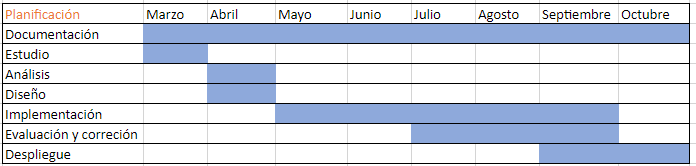
\includegraphics[width=1\textwidth]{imagenes/plan.png}
    \caption{ Planificación temporal }
    \label{fig:planificacion}
\end{figure}
\vspace{1cm}

\section{Presupuesto}

\subsection{Requerimientos software}

Todos los recursos software y tecnologías utilizadas en el proyecto son gratuitos. Partiendo desde el IDE utilizado en mi caso Visual Studio Code, como los framework Django y Foundation, Docker, todas las librerías, e incluso la conexión a la API de Telegram. Además se encuentra subido en un repositorio público de github, que nos ayuda a realizar copias y controlar versiones. 

El único gasto en recursos sería el despliegue del proyecto en un servidor. Si quisieramos migrarlo a la nube en Amazon Web Services un precio medio teniendo en cuenta varios factores como el tamaño de la instancia EC2, capacidad de almacenamiento de la base de datos y transferencia de datos nos costaría aproximadamente entre 40 y 70 euros por mes según \textit{(\cite{aws2022})}, que es lo que cuesta la arquitectura más básica. 

Cabe destacar que Amazon cobra toda la transferencia de datos que sucede por fuera de su misma red, es decir, cada dato que nosotros queramos mover dentro y fuera de AWS nos costará.


\subsection{Recursos humanos}


Teniendo en cuenta que este proyecto es desarrollado única y exclusivamente por mí, el coste de recursos humanos, contando las horas efectivas trabajadas en el proyecto por el autor y estableciendo un salario base de un programador de unos 14,62€ la hora según  \textit{(\cite{salario2022})} sería el siguiente:\vspace{0.5cm}


\begin{table}[!ht]
    \begin{center} 
    \begin{tabular}{| c | c | c |}
    \hline
    \rowcolor{blueice}
    Actividad & Horas & Coste  \\ \hline
    Análisis y diseño & 25h & 365€\\
    Implementación & 200h &  2924€\\
    Evaluación y corrección & 80h & 1169€ \\ \
    Despliegue & 10h & 146€ \\ 
    Documentación & 50h & 731€ \\ \hline
    \rowcolor{gray30}
    Total & 365h & 5336€ \\ \hline
    \end{tabular}
    \caption{Tabla presupuesto}
    \label{tab:presupuesto}
    \end{center}
\end{table}


